\documentclass{article} % For LaTeX2e
\usepackage{nips15submit_e}
\usepackage{hyperref}
\usepackage{url}
\usepackage{float}
\usepackage{graphicx}
\usepackage{caption}
\usepackage{subcaption}
\usepackage{capt-of}
%\documentstyle[nips14submit_09,times,art10]{article} % For LaTeX 2.09


\title{Making Music with Hidden Markov Models}


\author{
Anna Yanchenko \\
Duke University\\
\texttt{anna.yachenko@duke.edu} \\
\And
Megan Robertson \\
Duke University \\
\texttt{megan.robertson@duke.edu} \\
}


\newcommand{\fix}{\marginpar{FIX}}
\newcommand{\new}{\marginpar{NEW}}

\nipsfinalcopy % Uncomment for camera-ready version

\begin{document}


\maketitle

\begin{abstract}
We use Hidden Markov Models (HMM) to capture the latent elements involved in music creation. The observed states are the notes and velocity, volumes, of each note. The latent states include elements such as chord progression, dynamics and patterns.In this paper, we implement three different Hidden Markov Models and compare the resulting compositions for each model. These models are trained on various classical piano pieces, and the resulting compositions are compared.
\end{abstract}
 
\section{Introduction}

Hidden Markov Models are known for their use in language applications such as speech recognition and handwriting recognition programs. However, it is also possible to use Hidden Markov Models in another language application, the language of music. This project serves as a platform to combine our shared interests of music and statistics. 

The project uses music data in the form of  Musical Instrument Digital Interface (MIDI) files. This interface creates a form of communication between computers and musical instruments that enables them to send instructions back and forth. MIDI files can contain multiple channels that store information about the notes and velocity of certain instruments. The files also contain information about when a particular note starts and stops. \footnote{MIDI Manufacturers Association, "An Introduction to MIDI"}. 

Any musician or student of music can tell you that there is more to composing music beyond stringing together some notes with a catchy rhtyhm. There are many things to consider such as chord progression, dynamics, and patterns. It is importnat for a composer to be fmant for a composer to be familar with things such as the Circle of Fifths. There are also different forms, sonata, rondo, blues and more, that can be used in the creation of music.\footnote{Music Composition for Dummies, \url{http://www.dummies.com/how-to/content/music-composition-for-dummies-cheat-sheet.html}}

However, the MIDI data does not capture all of the theory and ideas that create a composition. Therefore, we use Hidden Markov Models (HMMs) in order to capture both the observed states, the note/velocity information, as well as the latent variables, theory such as that described above. We utitilze three different HMMs and train them on classical piano pieces. The estimated parameters are then used to compose new pieces.


\section{Methods}

Three classical piano pieces were used to train each of the models. The songs were Gustav Holt's Jupiter from "The Planets", Johann Pachelbel's Canon, and NEW WORLD/CLAIRDELUN. The MIDI files for these songs were converted to Comma Separated Value (CSV) files.\footnote{This was done using a program found at \url{http://www.fourmilab.ch/webtools/midicsv/}} 

The classical pieces were used to estimate the respective parameters of the models described below. Once the parameters had been estimated, they were used to generate a new piece of music. This process generates a CSV file of the new composition, and this file is then converted to a MIDI file using the same program as above. The files can then be played on a synsthesizer or a program such as GarageBand.

The three models used are described in the subsections below. They are a first order HMM, a second order HMM, and a first order HMM with two hidden states. 

- Transition matrix is the only thing changing between these models

\subsection {Model 1: First Order Hidden Markov Model}

The simplest of the three models is the first order Hidden Markov Model. In this model, the observed values, $X_i$, are the notes and their velocity. The model has only one hidden state for each note/velocity pair, $Z_i$, and each hidden state only depends on the prior hidden state. 

\begin{figure}[H]
\centering
\caption{Graphical Model - First Order HMM}
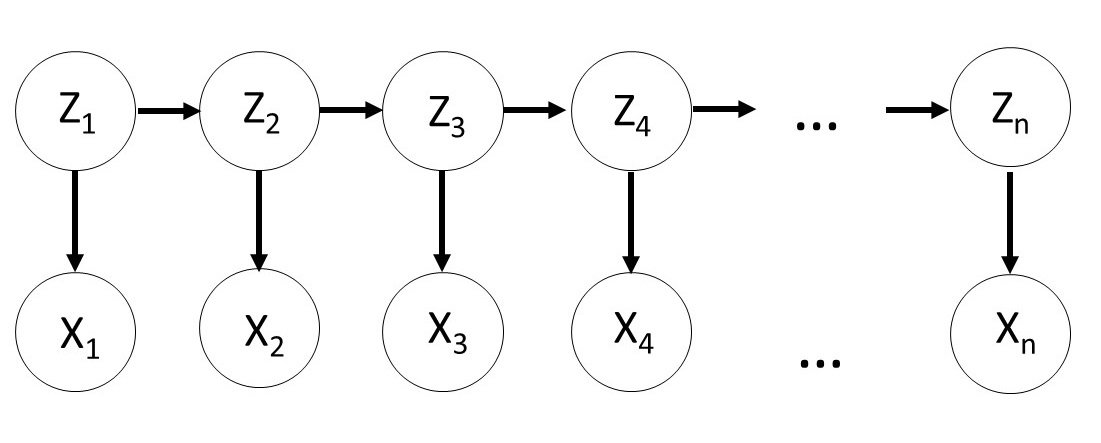
\includegraphics [scale = 0.35] {Model1.jpg}
\end{figure}

The Baum-Welch Alogirithm was used to estimate the parameters of this model. For details of the derivations and algorithm see class notes. \footnote{Statistics 531, Duke University Spring 2016. Instructor: Jeff Miller}
 
\subsection{Model 2: Second Order Hidden Markov Model}

The second model expanded on Model 1 by assuming that each state also depended on the prior two states. This enables the model to capture the structure that is evolving over time in the piece. The Baum-Welch Algorithm was again used to estimate the parameters. The details of the algorithm for this model can be found in Mari and Schott's "Probabilistic and Statsitical Methods in Computer Science." \footnote{Jean-Francoix Mari and Rene Schott, "Probabilistic and Statistical Methods in Computer Science", Springer Science, pg. 161-167 and Brett Watson and Ah Chung Tsoi, "Second Order Hidden Markov Models for Speech Recognition", Univsersity of Queensland}.

\begin{figure}[H]
\centering
\caption{Graphical Model - Second Order HMM}
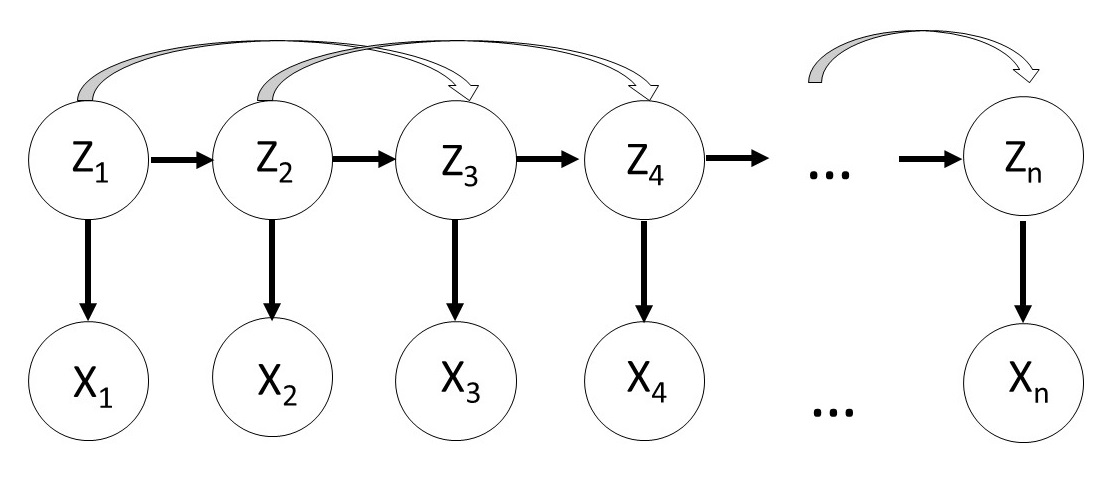
\includegraphics [scale = 0.35] {Model2.jpg}
\end{figure}

\subsection{Model 3: HMM with Two Hidden States}

The final model expanded on the intital model by adding a second latent variable. This meta-state allows the model to capture additional aspects of the hidden states and the music generation process.  This processes might evolve at a rate different than the processes that are present in the observed states and one latent state. 

\begin{figure}[H]
\centering
\caption{Graphical Model - First Order HMM with Two Hidden States}
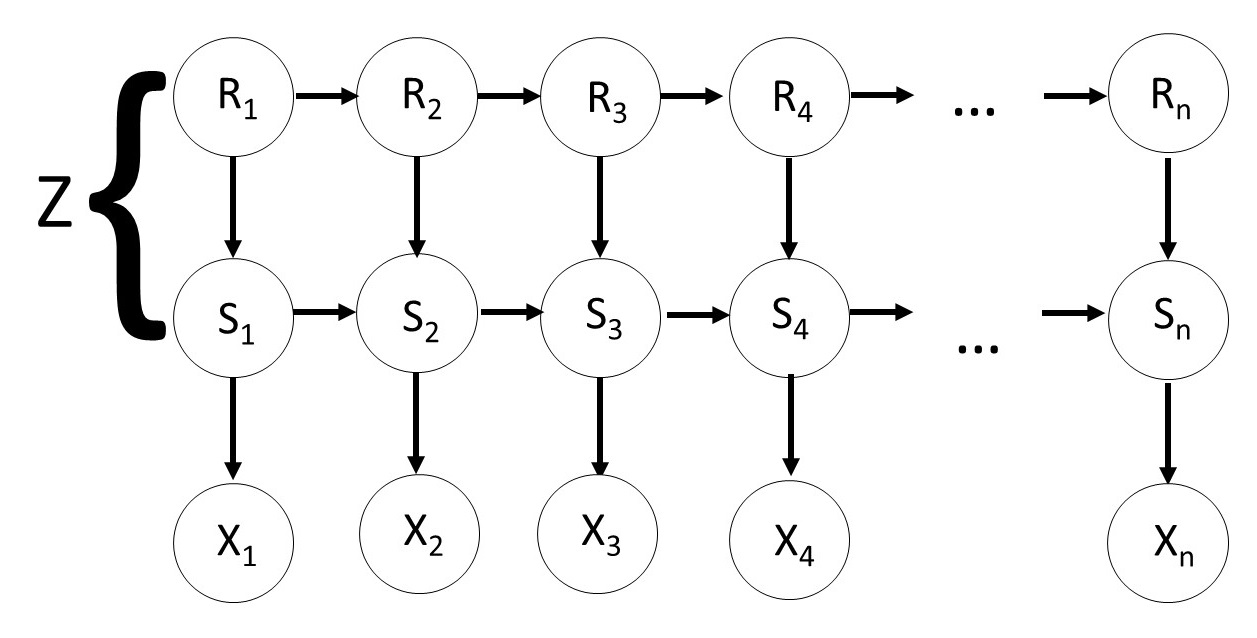
\includegraphics [scale = 0.35] {Model3.jpg}
\end{figure}

For the derivation of the Baum-Welch algorithm for this model, see the Appendix.

\section{Results}


\newpage

\section{Appendix}

\subsection{Baum-Welch for First Order HMM with Two Hidden States}

LATEX THIS HERE

\newpage

\section{References}
\begin{enumerate}
\item Wattson, Brett and Ah Chung Tsoi. "Second Order Hidden Markov Models for Speech Recognition", University of Queensland, 146-151. 
\item MIDI Manufacturers Association, "An Introduction to Midi". 
\item Music Composition for Dummies, http://www.dummies.com/how-to/content/music-composition-for-dummies-cheat-sheet.html
\end{enumerate}

\end{document}